\mychapter{Introduction}{Introduction}{}
\label{chap:introduction}

\mysection{Problem Background}{Problem Background}
\label{sec:overview}

- Satellites are getting smaller
- Because this leads to stallites having reduced costs and timelines
- This is enables by the miniraturisation of electronics

- One of the big industires in satellites is remote sensing
- Remote Sening is the application where satellites are used to monitor the Earth
- One of the applications is to take images of the Earth

- This leads to the problem that high accuracy is needed to take images of the targets on the Earth's surface
- COTS components which is mainly used on small satellites lack the accuracy needed
- Magnetometers is to low of an accuracy
- Star Trackers have the right accuracy, but is expensive

\mysection{Problem Definition}{Problem Defintion}
\label{sec:moddef}

A satellite orbiting Earth in the Earth-Centered Inertial (ECI) reference frame performs Earth observation missions, 
continuously capturing high-resolution imagery of the planet's surface for scientific, commercial, or operational purposes. 
To fulfill mission objectives effectively, the satellite must provide not only high-quality imagery but also precise geographic 
information about observed areas. This requires accurate knowledge of the satellite's six-degree-of-freedom pose 
(three-dimensional position and three-dimensional attitude) relative to the ECI frame at the moment each image is captured.
\vspace{0.5cm}

\noindent Traditional satellite pose determination relies on external systems such as Global Navigation Satellite Systems (GNSS) 
and ground-based tracking networks. However, this thesis investigates an autonomous approach where the satellite performs 
"visual navigation" by identifying known ground features in its imagery and using these observations to determine its orbital 
state. The satellite essentially performs "reverse GPS" - instead of receiving position signals from space, it observes 
recognizable landmarks on Earth's surface and computes its pose from these visual references.
\vspace{0.5cm}

\noindent The core technical challenge lies in the transformation from raw imagery to precise pose estimates. This involves several 
interdependent problems: \textbf{(1) Feature Detection} - identifying which pixels in the imagery correspond to cataloged 
landmarks among millions of pixel observations; \textbf{(2) Geometric Inversion} - solving the complex inverse problem of 
determining six-dimensional pose from two-dimensional image projections of three-dimensional landmarks with known geographic 
coordinates; and \textbf{(3) Uncertainty Management} - handling measurement noise, feature detection errors, and dynamic orbital 
motion in real-time. This thesis assumes the availability of a pre-established catalog of ground features with precisely 
known geographic coordinates in the ECI frame. The feature matching problem - associating detected image features with specific 
catalog entries - is considered solved through prior knowledge of the observed terrain and existing geographic databases.
\vspace{0.5cm}

\begin{figure}[htbp]
    \centering
    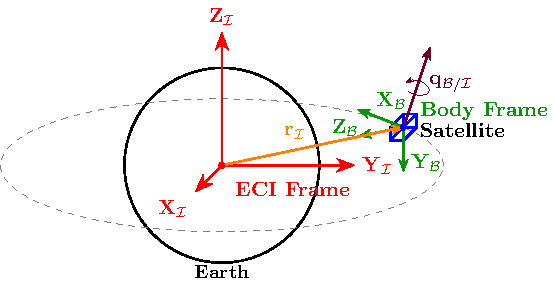
\includegraphics[width=0.8\textwidth]{figures/Figure1.pdf}
    \caption{Satellite pose estimation concept showing orbital geometry, reference frames}
    \label{fig:satellite_concept}
\end{figure}

This problem structure aligns with a simplified version of the Simultaneous Localization and Mapping (SLAM) framework. 
In this context, \textbf{localization} corresponds to determining the satellite's pose relative to the ECI frame using 
observations of cataloged features, while the \textbf{mapping} component is reduced to feature catalog utilization rather 
than creation. Since the geographic locations of observable features are assumed known a priori, the primary focus becomes the 
pose estimation problem given established feature correspondences.
\vspace{0.5cm}

The satellite's pose estimation system must account for the dynamic nature of orbital motion, 
the geometric relationship between the camera frame and satellite body frame, and the projection 
characteristics of the imaging system, while maintaining computational efficiency suitable for 
real-time onboard processing. 



\mysection{Proposed Solution}{Proposed Solution}
\label{sec:description}

- Proposed solution is to develop an estimation algorithm that can estimate the full state of the satellite
- The Full State of a Satellite is its postition in Space and its attitude or its orientation in space.
- The satellite uses the imager itself to determine position and attitude.
- This can lead to reduce costs as the satellite is using an instrument which is already onboard the satellite.
- Utilising the components when it is idle
- Observing the target directly


\mysection{Document Outline}{Document Outline}
\label{sec:outline}

- Chapter 2: Wil investigate previous sensors that is being used to determine Propose
- Previous techniques estimating the pose
- Some light touching on feature detection as this is crucial to the pose estimation system

- Chapter 3: Wil introduce the modelling of the system
- Rigid Body Kinematics
- Position Kinematics
- Attitude Kinematics
- Kalman Filters
- Extended Kalman Filters

- Chapter 4: Measurement Generation
- Feature detection
- PinHole Camera Model.
- The Plant
- The Plant Model
- The Measurment Model

- Chapter 5: State estimation
- The Extended Kalman Filter
- Update Step
- Prediction Step
- Simulator

- Chapter 6 is results

- Chapter 7 is Conclusion
- Future Work